\section{Suma de enteros en base dos}

%----------
% MT-2A
%----------

\subsection{MT Determinista de 1 cinta}

\subsubsection*{Diseño propuesto}
El algoritmo de resolución es el siguiente:

\begin{itemize}
    \item Ciclo:
    \begin{enumerate}[1.]
        \item Comienzo desde la izquierda, desplazamiento hasta el extremo derecho.
        \item Si el último elemento es un 1:
        \begin{enumerate}[1.]
            \item Borrarlo.
            \item Volver al extremo izquierdo.
            \item Añadir un 1 en la primera posición.
        \end{enumerate}
        \item Si el último elemento es un 0:
        \begin{enumerate}[1.]
            \item Borrarlo y sustituirlo por un 1.
            \item Volver hacia la izquierda.
            \item Si se encuentra un 1 
            \begin{enumerate}[1.] 
                \item sustituirlo por un 0
            \end{enumerate}
            \item Si se encuentra un 0
            \begin{enumerate}[1.]
                \item sustituirlo por un 1
                \item Si se encuntra un \$
                \begin{enumerate}[1.]
                    \item Avanzar hatsa el extremo derecho
                    \item Volver hacia la izquierda eliminando todo los elementos hasta el \$ incluido
                    \item \textbf{Parar}.
                \end{enumerate}
            \end{enumerate}
            \item \textbf{Parar}.
        \end{enumerate}
    \end{enumerate}
\end{itemize}

El diseño de la máquina queda representado en la Figura \ref{fig:MT-2A}.

\begin{figure}[h]
    \centering
    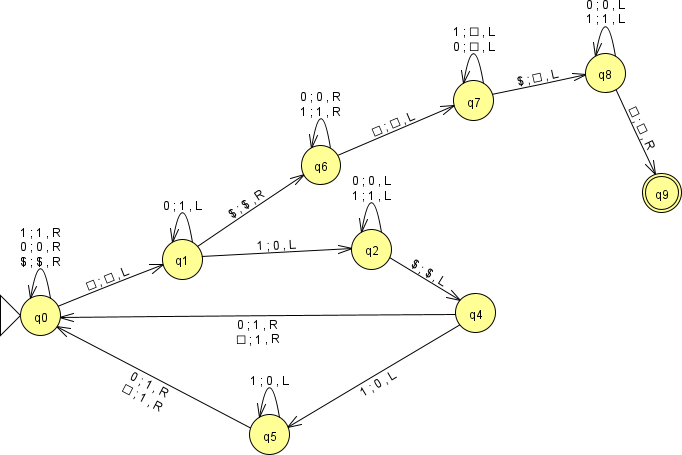
\includegraphics[width=0.6\textwidth]{MT-2A.png}
    \caption{Implementación en JFLAP de MT-2A}
    \label{fig:MT-2A}
\end{figure}


\subsubsection*{Peor caso}
Dado que la maquina funciona restando de uno en uno al número de la derecha y sumando en la misma medida al número de de la izquierda, el peor caso será aquel en el que se requieran llevar acabo más acarreo de bits puesto que esto implica modificar el valor de todos los digitos del número al que se le está sumando. Esto ocurrirá para un mismo número de dígitos el número de 1 sea mayor, decir a mayor número de dgitos con valor 1 más ciclos se requerirán.\\
Del mismo modo al restar a la derecha para sumar a la izquierda, a más digitos en la derecha más ciclos de suma-resta se reuerirán.

\subsubsection*{Evaluación empírica}
Realizamos la evaluación empírica en el peor caso, tomando como $n$ el tamaño de la cadena de entrada, compuesta por por 1 a la derecha del \$ ya que se trataría del peor caso, y midiendo el número de pasos realizados para resolver el problema\footnote{Los datos se pueden encontrar en \texttt{data/MT-2A.csv}.}:

\begin{table}[h]
    \centering
    \begin{tabular}{lccc}
        Entrada & $n_d$ & Pasos \\
        \hline
        \$1                     & 2  & 17   \\
        \$11                    & 3  & 42   \\
        \$111                   & 4  & 99  \\
        \$1111                  & 5  & 228  \\
        \$11111                 & 6  & 517  \\
    \end{tabular}
\end{table}


\subsubsection*{Coste computacional}
Para obtener el coste computacional del algoritmo, aplicaremos Diferencias Finitas, basándonos en los datos de la evaluación empírica:


\begin{table}[h]
    \centering
    \begin{tabular}{|l|c|c|c|c|c|c|c|}
        \hline
        $n$ & \textbf{2} & \textbf{3} & \textbf{4} & \textbf{5} & \textbf{6}\\ \hline
        $T(n)$ & \textbf{17} & \textbf{42} & \textbf{99} & \textbf{228} & \textbf{517}      \\ \hline
        \hline
        $A(n) = T(n) - T(n-2)$ &    & 25 & 57 & 129 & 289 \\ \hline
        $B(n) = A(n) - A(n-2)$ &    &   & 32 & 72 & 160 \\ \hline
        $C(n) = B(n) - B(n-2)$ &    &   &    & 40 & 88 \\ \hline
    \end{tabular}
\end{table}

Se obsrerva que ni las diferencias finitas primeras ni las segundas o terceras son no nulas, esto se debe a que el funcionamiento de la máquina de Turing es recursivo, por lo que no es posible aproximarlo a un polinomio con exactitud\\


%----------
% MT-2B
%----------


\subsection{MT Determinista de 2 cintas}

\subsubsection*{Diseño propuesto}
El algoritmo de resolución es el siguiente:

\begin{itemize}
    \item Ciclo:
    \begin{enumerate}[1.]
        \item Comienzo desde la izquierda, desplazamiento hasta el extremo derecho.
        \item Si el último elemento es un 1:
        \begin{enumerate}[1.]
            \item Borrarlo.
            \item Volver al extremo izquierdo.
            \item Añadir un 1 en la primera posición.
        \end{enumerate}
        \item Si el último elemento es un 0:
        \begin{enumerate}[1.]
            \item Borrarlo y sustituirlo por un 1.
            \item Volver hacia la izquierda.
            \item Si se encuentra un 1 
            \begin{enumerate}[1.] 
                \item sustituirlo por un 0
            \end{enumerate}
            \item Si se encuentra un 0
            \begin{enumerate}[1.]
                \item sustituirlo por un 1
                \item Si se encuntra un \$
                \begin{enumerate}[1.]
                    \item Avanzar hatsa el extremo derecho
                    \item Volver hacia la izquierda eliminando todo los elementos hasta el \$ incluido
                    \item \textbf{Parar}.
                \end{enumerate}
            \end{enumerate}
            \item \textbf{Parar}.
        \end{enumerate}
    \end{enumerate}
\end{itemize}

El diseño de la máquina queda representado en la Figura \ref{fig:MT-2B}.

\begin{figure}[h]
    \centering
    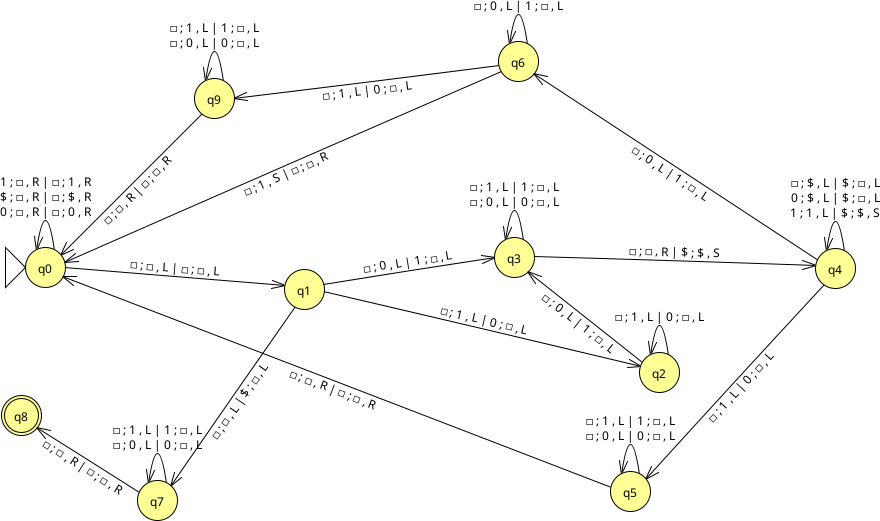
\includegraphics[width=0.6\textwidth]{MT-2B.png}
    \caption{Implementación en JFLAP de MT-2B}
    \label{fig:MT-2B}
\end{figure}